\pagebreak
\section{Scope and Content of this Document}
The GDS Technical Specification is written for those wishing to create or use any GHRSST product
and requiring detailed technical information on their contents and specifications. It provides the
technical specifications for all GHRSST data sets used within the GHRSST Regional/Global Task
Sharing (R/GTS) Framework. An overview of GHRSST and the GDS presented followed by a detailed
technical specification of the GHRSST file naming specification, supporting definitions and
conventions. The technical specifications for all GHRSST Level 2P (L2P), Level 3 (L3), Level 4 (L4),
and GHRSST Multi-Product Ensemble (GMPE) data products are then provided. The GDS also
provides code tables and best practices for identifying sources of SST and ancillary data within
GHRSST data files.\par\vspace{0.25cm}
\noindent This document has been developed for data providers who wish to produce any level of GHRSST
data product and for all users wishing to fully understand the file naming convention, GHRSST data
file contents, GHRSST and Climate Forecast definitions for SST, and other useful information.
Additional information describing GHRSST and its component international services is available at
\url{http://www.ghrsst.org} and many relevant GHRSST web sites are listed on the last page of this
document.\par\vspace{0.25cm}
\noindent The GDS Technical Specification document forms a component document of the GDS 2.0 document
set, which is shown schematically in Figure 5-1 below. Other documents from the GDS 2.0 document
pack that are specified in the Applicable Documents section of this document shall be consulted when
using this document. \par\vspace{0.25cm}
\begin{figure}[h]
    \centering
    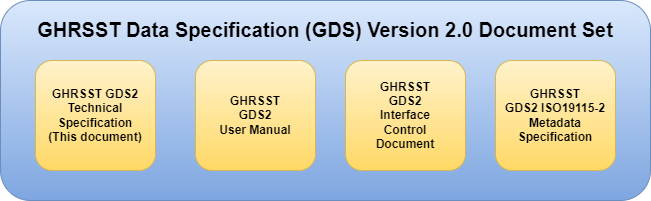
\includegraphics[width=1 \textwidth]{../images/schematicOverview.drawio.png}
    \caption{Schematic overview of the GHRSST Data Specification Version 2.0 document pack.}
    \label{fig:schematic_overview}
\end{figure}